\documentclass[aspectratio=169]{beamer}
\usepackage[utf8]{inputenc}
\usepackage{booktabs}
\usepackage{graphicx}
\usepackage{xcolor}

% Color Definitions
\definecolor{NVIDIAGreen}{RGB}{118, 185, 0}
\definecolor{DarkGrey}{RGB}{30, 30, 30}
\definecolor{LightGrey}{RGB}{240, 240, 240}

% Beamer Theme Settings
\usetheme{Madrid}
\usecolortheme{default}

% Customize Colors
\setbeamercolor{palette primary}{bg=DarkGrey, fg=white}
\setbeamercolor{palette secondary}{bg=NVIDIAGreen, fg=white}
\setbeamercolor{palette tertiary}{bg=DarkGrey, fg=white}
\setbeamercolor{titlelike}{parent=palette primary, fg=NVIDIAGreen}
\setbeamercolor{structure}{fg=NVIDIAGreen}
\setbeamercolor{item}{fg=NVIDIAGreen}

% Title Slide Info
\title[NVIDIA cuOpt]{NVIDIA cuOpt}
\subtitle{GPU-Accelerated Decision Optimization}
\author{Huutrungle2001}
\date{\today}

\begin{document}

% Slide 1: Title
\begin{frame}
    \titlepage
\end{frame}

% Slide 2: The Core Challenge
\begin{frame}{The Core Challenge: Decision Bottlenecks}
    \begin{itemize}
        \item \textbf{High Complexity:} Real-world logistics, supply chains, and portfolio management contain millions of variables and constraints.
        \item \textbf{Latency Barriers:} Traditional CPU solvers take hours to calculate optimal solutions, making real-time, dynamic decision-making impossible.
        \item \textbf{Operational Costs:} High solve times directly translate to elevated fuel waste, idle vehicle fleets, and inefficient resource allocation.
    \end{itemize}
\end{frame}

% Slide 3: What is NVIDIA cuOpt?
\begin{frame}{What is NVIDIA cuOpt?}
    NVIDIA\textsuperscript{\textregistered} cuOpt\textsuperscript{\texttrademark} is an open-source, GPU-accelerated optimization engine.
    \vspace{0.3cm}
    \begin{columns}
        \begin{column}{0.5\textwidth}
            \textbf{Supported Mathematical Models:}
            \begin{itemize}
                \item Linear Programming (LP/PDLP)
                \item Mixed-Integer Programming (MIP) \textit{[Beta]}
                \item Quadratic Programming (QP)
            \end{itemize}
            \vspace{0.2cm}
            \textbf{Routing Specialization:}
            \begin{itemize}
                \item Traveling Salesperson (TSP)
                \item Vehicle Routing Problems (VRP)
            \end{itemize}
        \end{column}
        \begin{column}{0.5\textwidth}
            \centering
            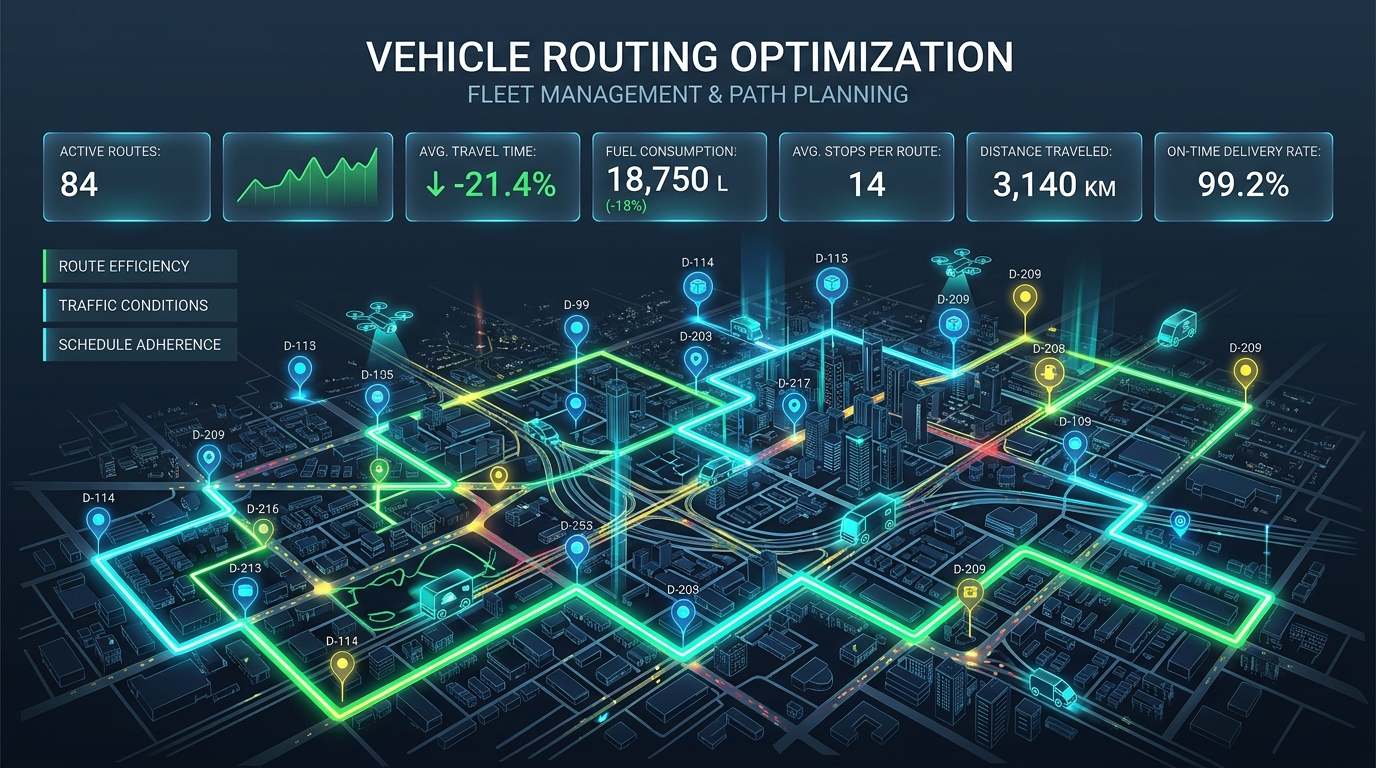
\includegraphics[width=\textwidth]{images/routing_optimization.png}
        \end{column}
    \end{columns}
\end{frame}

% Slide 4: Hybrid GPU/CPU Primal Heuristics
\begin{frame}{Hybrid GPU/CPU Primal Heuristics}
    \begin{itemize}
        \item \textbf{GPU Offloading:} Offloads math-heavy \textbf{primal heuristics} (Feasibility Pump/Jump, Fix-and-Propagate) to thousands of parallel GPU cores.
        \item \textbf{CPU Tree Search:} Integrates with traditional CPU methods to perform dual-bound computations and branch-and-bound pruning.
        \item \textbf{Performance Gain:} Achieves up to \textbf{5,000x speedups} on large LP benchmarks and resolves objective gaps on MIPs at world-record speed.
    \end{itemize}
\end{frame}

% Slide 5: Real-World Use Cases: Logistics & Routing
\begin{frame}{Real-World Use Cases: Logistics \& Routing}
    \begin{columns}
        \begin{column}{0.5\textwidth}
            \begin{itemize}
                \item \textbf{Last-Mile Delivery:} Optimizes routing paths to reduce fuel consumption and transit mileage (e.g., Azure Maps Integration).
                \item \textbf{Fleet Management:} Coordinates long-haul inbound/outbound transport, resting constraints, and schedules.
                \item \textbf{Omniverse Digital Twins:} Simulates physical factory warehouses in virtual environments for optimized intralogistics (e.g., BMW, SyncTwin).
            \end{itemize}
        \end{column}
        \begin{column}{0.5\textwidth}
            \centering
            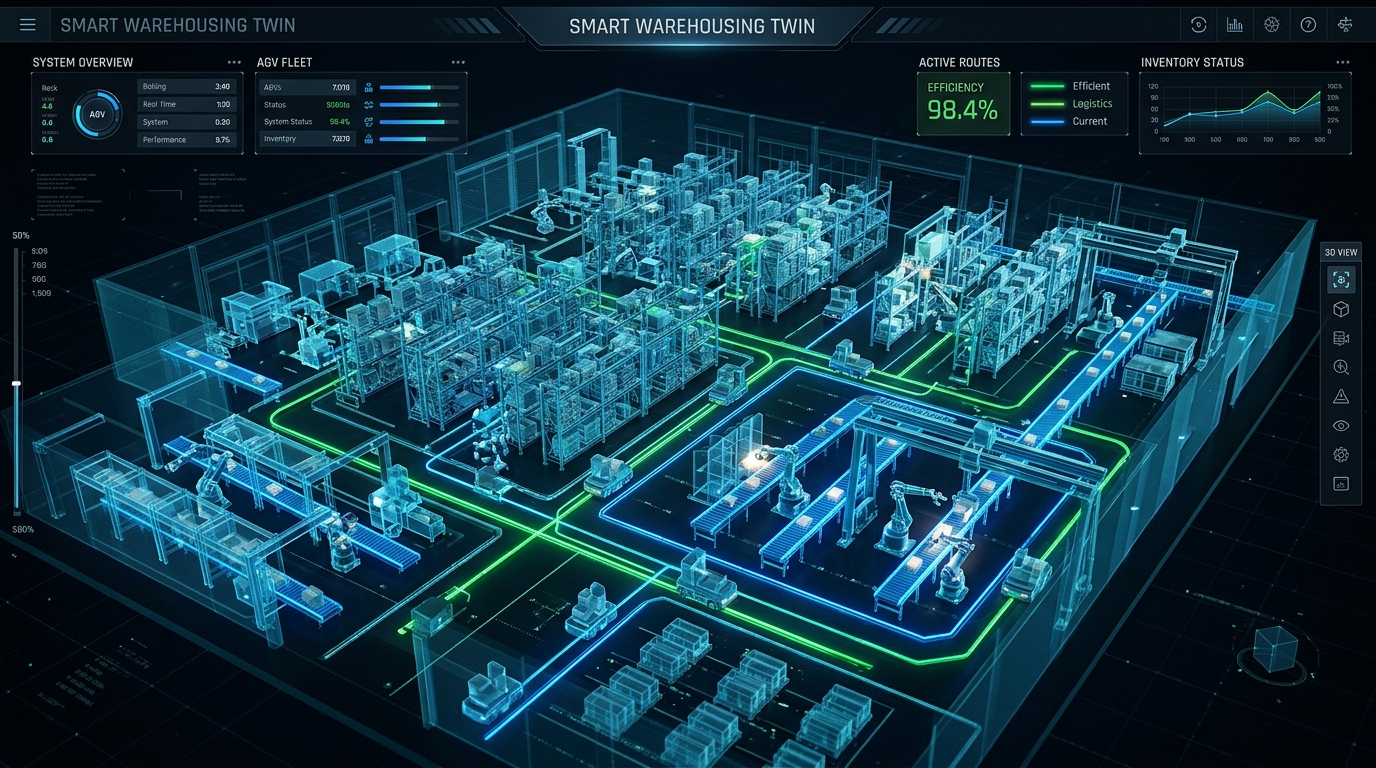
\includegraphics[width=\textwidth]{images/logistics_twin.png}
        \end{column}
    \end{columns}
\end{frame}

% Slide 6: Real-World Use Cases: Scheduling \& Finance
\begin{frame}{Real-World Use Cases: Scheduling \& Finance}
    \begin{itemize}
        \item \textbf{Job Scheduling:} Dynamically assigns tasks to workers, machinery, or computing networks to optimize factory throughput. Runs near real-time re-optimizations when machines breakdown.
        \item \textbf{Portfolio Optimization:} Accelerates large-scale Quadratic Programming (QP) to rebalance financial assets instantly based on high-frequency market updates.
    \end{itemize}
\end{frame}

% Slide 7: Next-Gen AI Agent Integration
\begin{frame}{Next-Gen AI Agent Integration}
    \begin{itemize}
        \item \textbf{cuOpt Agent Skills:} Open-source, modular skills compatible with common agent frameworks.
        \item \textbf{Natural Language Interfaces:} Translates plain English business constraints directly into optimization models.
        \item \textbf{Skill Cards:} Machine-readable cards providing clear documentation, security parameters, and performance validation.
    \end{itemize}
\end{frame}

% Slide 8: Getting Started \& Scale Tiers
\begin{frame}{Getting Started \& Scale Tiers}
    \centering
    \begin{tabular}{llcl}
        \toprule
        \textbf{Access Tier} & \textbf{Limits} & \textbf{Integrations} & \textbf{Target Use Case} \\
        \midrule
        API Catalog & Up to 1,000 nodes & REST API & Free prototyping \\
        Google Colab & Free GPU Sandbox & Python API & Quick experimentation \\
        Local Dev & Custom single-GPU & Pip/Conda/Docker & Developer builds \\
        Enterprise & 15,000+ nodes & AI Enterprise & Mission-critical production \\
        \bottomrule
    \end{tabular}
    \vspace{0.4cm}
    \begin{itemize}
        \item Seamless modeling integrations with \textbf{AMPL, CVXPY, PuLP, JuMP, and GAMSPy}.
    \end{itemize}
\end{frame}

% Slide 9: Conclusion
\begin{frame}{Conclusion}
    \centering
    \Huge \textcolor{NVIDIAGreen}{\textbf{Thank You!}} \\
    \vspace{0.5cm}
    \Large \textcolor{black}{Questions \& Answers} \\
    \vspace{0.8cm}
    \small \href{https://www.nvidia.com/en-us/ai-data-science/products/cuopt/}{nvidia.com/cuopt}
\end{frame}

\end{document}
